\subsection{Sets}
\begin{definition}
    An unordered collection of objects (i.e. elements or members)
    \begin{itemize}
        \item A set \emph{contains} its elements or elements of a set are \emph{contained in} that set.
    \end{itemize}
\end{definition}

    \subsubsection{Set notation}
    \begin{terminology}
        \begin{itemize}
            \item $\ldots$ mean "and so on"
            \item $:$ mean "such that"
            \item $\in$ mean "contained"
            \item $\notin$ mean "not contained"
            \item $\emptyset$ mean "empty set (i.e. a set contains no elements")
            \item $A\subseteq B$ mean "Only if every element of $A$ is also an element of $B$"
            \item $B\supseteq A$ mean "B is a superset of A to mean A is a subset of B" 
            \item Normally, elements of a set are listed just once.
        \end{itemize}
    \end{terminology}

\begin{example}

    \textbf{Sets:}
    \begin{itemize}
        \item $E = \{0,2,4,6,8\}$, where $2\in E$ and $1 \notin E$
        \item $\mathbb{Z} = \{\ldots,-2,-1,0,1,2,\ldots\}$
        \item $P=\{0,1,...,255\}$
        \item $O = \{x \in \mathbb{Z}: \; x=2k+1 \text{ for some } k \in \mathbb{Z}\}$
        \item $\{\emptyset,\{\emptyset\}\}$ (i.e. A set that has other sets as elements).
    \end{itemize}
    \vspace{1em}

    \textbf{Subset:}
    \begin{itemize}
        \item $E \subseteq \mathbb{Z}$
    \end{itemize}
\end{example}

\begin{theorem}
    $A = B$ means $A \subseteq B$ and $B \subseteq A$.
    \begin{itemize}
        \item \textbf{Note:} Have to prove in both directions.
    \end{itemize}
\end{theorem}

\begin{example}
    $\{1,2,3\}=\{3,2,1,1,2\}$
\end{example}

    \subsubsection{Important sets}
    \begin{definition}
        \begin{enumerate}
            \item \textbf{Natural:} \( \mathbb{N} = \{0, 1, 2, 3, \dots \} \): 
            \item \textbf{Integers:} \( \mathbb{Z} = \{ \dots, -2, -1, 0, 1, 2, \dots \} \): 
            \item \textbf{Rational:} \( \mathbb{Q} = \left\{ \frac{a}{b} : a, b \in \mathbb{Z}, b \neq 0 \right\} \): 
            \item \textbf{Real:} \( \mathbb{R} \): 
            \item \textbf{Complex:} \( \mathbb{C} = \{ a + bj : a, b \in \mathbb{R} \} \)
            \begin{itemize}
                \item \( j \): imaginary unit, where \( j^2 = -1 \) and \( j = \sqrt{-1} \)
            \end{itemize}
        \end{enumerate}  
        \begin{itemize}
            \item \textbf{Note:} $\mathbb{N} \subseteq \mathbb{Z} \subseteq \mathbb{Q} \subseteq \mathbb{R} \subseteq \mathbb{C} $
        \end{itemize}      
    \end{definition}

\subsection{Ordered n-tuples}
\begin{definition}
    An ordered collection of \( n \) elements, where \( n \) is a positive integer, denoted as \( (a_1, a_2, \dots, a_n) \), where \( a_1 \) is the first element, and so on, up to \( a_n \).
\end{definition}
    
    \subsubsection{How are two tuples equal?}
    \begin{definition}
        Unlike sets, both the order of elements and the repetition of values are significant. Therefore, two ordered \( n \)-tuples are considered equal (i.e. $(a_1, a_2, \dots, a_n) = (b_1, b_2, \dots, b_n)$) iff:

        \[
        a_1 = b_1, a_2 = b_2, \dots, a_n = b_n.
        \]
    \end{definition}

    \subsubsection{Cartesian product}
    \begin{definition}
        \textbf{Two sets:}
        The \textit{Cartesian product} of two sets \( A \) and \( B \) (in that order), denoted as \( A \times B \), is the set of all \textit{ordered pairs} or \textit{ordered 2-tuples} \( (a, b) \) where \( a \in A \) and \( b \in B \). Thus

        \begin{equation}
            A \times B = \{ (a, b) : a \in A, b \in B \}.    
        \end{equation}
        \begin{itemize}
            \item \textbf{General:} $B \times A \neq A \times B$
            \item \textbf{2-fold Cartesian product:} $A \times A$ is denoted as $A^2$
        \end{itemize}
        \vspace{1em}

        \textbf{More than two sets:}
        The Cartesian product of sets \( A_1, A_2, \dots, A_n \), denoted as \( A_1 \times A_2 \times \cdots \times A_n \), is the set of ordered \( n \)-tuples \( (a_1, a_2, \dots, a_n) \), where \( a_1 \in A_1, a_2 \in A_2, \dots, a_n \in A_n \). Thus

        \begin{equation}
            A_1 \times A_2 \times \cdots \times A_n = \{(a_1, a_2, \dots, a_n) : a_1 \in A_1, a_2 \in A_2, \dots, a_n \in A_n\}.
        \end{equation}
        \begin{itemize}
            \item \textbf{n-fold Cartesian product:} $A\times A\times \cdots \times A$ is denoted as $A^n$
        \end{itemize}

    \end{definition}

\subsection{Functions}
\begin{definition}
    A function \( f: A \to B \) from a set \( A \) (the domain of \( f \)) to a set \( B \) (the codomain of \( f \)) assigns to each element \( a \in A \) exactly one element \( b \in B \), usually denoted as \( b = f(a) \).
\end{definition}

    \subsubsection{Range/Image}
    \begin{definition}
        \textbf{The range or image} of \( f \) is the subset of the codomain $B$ given as 
        \[
        \text{Im}_f(A) = \{ b \in B: \exists a \in A(f(a) = b) \}.
        \]
        \begin{itemize}
            \item \textbf{English:} Set of values "hit" by $f$ as its argument ranges over the set $A$.
        \end{itemize}
    \end{definition}

    \subsubsection{Inverse Image}
    \begin{definition}
        \textbf{The inverse image or pre-image} of any element \( b \in B \) under the mapping by \( f \) is the set 
        \[
        f^{-1}(b) = \{ a \in A : f(a) = b \}.
        \]
        \begin{itemize}
            \item \textbf{English:} Set of elements of the domain that map to $b$ under transformation by $f$.
            \item \textbf{Key:} If $b$ is an element of the codomain that is not in the range of $f$, then $f^{-1} (b) = \emptyset$
        \end{itemize}
    \end{definition}

\begin{example}
    \begin{itemize}
        \item Domain of \( g \): \( A = \{ 1, 2, 3, 4 \} \)
        \item Codomain of \( g \): \( B = \{ w, x, y, z \} \)
        \item Image of \( A \): \( \text{Im}_g(A) = \{ w, x, z \} \subseteq B \)
        \item Inverse Image
        \[
        g^{-1}(w) = \{ 1 \}
        \]
        \[
        g^{-1}(x) = \{ 2, 4 \}
        \]
        \[
        g^{-1}(y) = \emptyset
        \]
        \[
        g^{-1}(z) = \{ 3 \}
        \]
    \end{itemize}
    
    % Mapping Diagram
    \begin{center}
    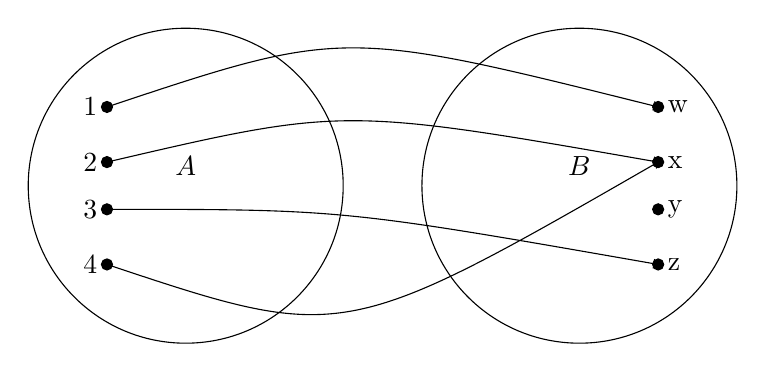
\begin{tikzpicture}
        % Sets A and B
        \draw (0, 0) circle (2cm) node[anchor=south] {$A$};
        \draw (5, 0) circle (2cm) node[anchor=south] {$B$};
    
        % Elements in A
        \filldraw[black] (-1, 1) circle (2pt) node[anchor=east] {1};
        \filldraw[black] (-1, 0.3) circle (2pt) node[anchor=east] {2};
        \filldraw[black] (-1, -0.3) circle (2pt) node[anchor=east] {3};
        \filldraw[black] (-1, -1) circle (2pt) node[anchor=east] {4};
    
        % Elements in B
        \filldraw[black] (6, 1) circle (2pt) node[anchor=west] {w};
        \filldraw[black] (6, 0.3) circle (2pt) node[anchor=west] {x};
        \filldraw[black] (6, -0.3) circle (2pt) node[anchor=west] {y};
        \filldraw[black] (6, -1) circle (2pt) node[anchor=west] {z};
    
        % Arrows for mappings
        \draw[->] (-1, 1) .. controls (2, 2) .. (6, 1);  % 1 -> w
        \draw[->] (-1, 0.3) .. controls (2, 1) .. (6, 0.3);  % 2 -> x
        \draw[->] (-1, -0.3) .. controls (2, -0.3) .. (6, -1);  % 3 -> z
        \draw[->] (-1, -1) .. controls (2, -2) .. (6, 0.3);  % 4 -> x
    \end{tikzpicture}
    \end{center}    
\end{example}

    \subsubsection{Injective}
    \begin{definition}
        A function \( f: A \to B \) is called injective (or an injection or one-to-one) if $\forall a_1 \forall a_2$
        \[
        a_1 \neq a_2 \rightarrow f(a_1) \neq f(a_2).
        \]
        \[
        (f(a_1) = f(a_2) \rightarrow a_1 = a_2)
        \]

        \begin{itemize}
            \item \textbf{English:} Maps distinct elemetns of the domain to distinct elements of the codomain.
        \end{itemize}
        \customFigure[0.25]{00_Images/Injective.png}{Injective function.}
    \end{definition}

    \begin{process}
        Show a function is injective:
        \begin{enumerate}
            \item Set $f(x_1) = f(x_2)$
            \item Prove $x_1 = x_2$ from step 1. 
        \end{enumerate}
        \vspace{1em}

        Show a function is not injective:
        \begin{enumerate}
            \item Find a counterexample where $f(a_1) = f(a_2)$.
        \end{enumerate}
    \end{process}

    \subsubsection{Surjective}
    \begin{definition}
        A function \( f: A \to B \) is called surjective (or a surjection or onto) if 
        \[
        \forall b (f^{-1}(b) \neq \emptyset), \quad \text{or} \quad \forall b \exists a (f(a) = b),
        \]
        \begin{itemize}
            \item \textbf{English:} Every element in the codomain has a mapping back to the domain.
        \end{itemize}

        \customFigure[0.25]{00_Images/Surjective.png}{Surjective function.}
    \end{definition}

    \begin{process}
        Show a function is surjective:
        \begin{enumerate}
            \item Find the inverse of $f(x)=y$ by writing $x$ in terms of $y$ denoted $f^{-1}$
            \item See if the inverse satisfies the codomain, and there is no empty set.
        \end{enumerate}
        \vspace{1em}

        Show a function is not surjective:
        \begin{enumerate}
            \item Find a counterexample, where you get the empty set for $b\in B$
        \end{enumerate}
    \end{process}

    \begin{warning}
        Any nonsurjective function is a surjective function obtained from the original function by having the codomain match the range.
    \end{warning}

    \subsubsection{Bijective}
    \begin{definition}
        A function \( f: A \to B \) that is both injective and surjective is called bijective (or a bijection or a one-to-one correspondence).
        \begin{itemize}
            \item \textbf{Correspondence:} Inverse exists
        \end{itemize}
        \customFigure[0.25]{00_Images/Bijective.png}{Bijective function.}
    \end{definition}

    \subsubsection{Composition of g with f}
    \begin{definition}
        If \( f: A \to B \) and \( g: B \to C \), then \( g \circ f: A \to C \) s.t. $a \rightarrow g(f(a))$ (i.e. first apply $f$, then apply $g$)
        
        \customFigure[0.5]{00_Images/Composition.png}{Composition example}
        \begin{itemize}
            \item \textbf{Order is important:} $ f(g(a)) \neq g(f(a)) $
        \end{itemize}
    \end{definition}

    \subsubsection{Identity map}
    \begin{definition}
        \[
        \text{id}_A: A \to A \quad \text{id}(a) = a \; \forall a \in A
        \]
    \end{definition}

    \subsubsection{Bijective property}
    \begin{definition}
        Let \( f: A \to B \), then iff \( f \text{ is bijective, } \exists \text{ a function } f^{-1}: B \to A \text{ s.t. } f^{-1} \circ f = \text{id}_A \text{ and } f \circ f^{-1} = \text{id}_B \).
        \customFigure[0.5]{00_Images/Bijective_Property.png}{Illustration of bijective function}
    \end{definition}

    \subsubsection{Set of all functions with domain and codomain}
    \begin{definition}
        The set of all fcns with domain $A$ and codomain $B$ is itself a set denoted $B^A$.
    \end{definition}

\begin{example}
    % Example of the set of all functions from A to B
    If \( A = \{1, 2\} \) and \( B = \{x, y, z\} \), then \( B^A \) has \( 3^2 = 9 \) elements (i.e., \( B^A \)).

    \[
    f = \left( \begin{array}{c c}
    1 & 2 \\
    f(1) & f(2) \\
    \end{array} \right)
    \]

    The set \( B^A \) is:

    \[
    B^A = \left\{
    \left( \begin{array}{c c}
    1 & 2 \\
    x & x \\
    \end{array} \right),
    \left( \begin{array}{c c}
    1 & 2 \\
    x & y \\
    \end{array} \right),
    \left( \begin{array}{c c}
    1 & 2 \\
    x & z \\
    \end{array} \right),
    \left( \begin{array}{c c}
    1 & 2 \\
    y & x \\
    \end{array} \right),
    \left( \begin{array}{c c}
    1 & 2 \\
    y & y \\
    \end{array} \right),
    \left( \begin{array}{c c}
    1 & 2 \\
    y & z \\
    \end{array} \right),
    \left( \begin{array}{c c}
    1 & 2 \\
    z & x \\
    \end{array} \right),
    \left( \begin{array}{c c}
    1 & 2 \\
    z & y \\
    \end{array} \right),
    \left( \begin{array}{c c}
    1 & 2 \\
    z & z \\
    \end{array} \right)
    \right\}
    \]
\end{example}

\subsection{Complex math}
    \subsubsection{Complex number basics}
    \begin{definition}
    \begin{itemize}
        \item \( z = a + bj \), where \( a, b \in \mathbb{R} \)
        \begin{itemize}
            \item \( \text{Re}(z) = a \)
            \item \( \text{Im}(z) = b \)
        \end{itemize}
        
        \item \textbf{Complex conjugate:} If \( z = a + bj \), then \( z^* = a - bj \).
        
        \item \textbf{Magnitude:} \( |z| = \sqrt{z \cdot z^*} = \sqrt{a^2 + b^2} \).
    \end{itemize}

        % Complex plane diagram
        \begin{center}
        \begin{tikzpicture}
            \draw[->] (-0.5, 0) -- (3, 0) node[anchor=north] {$Re$};
            \draw[->] (0, -0.5) -- (0, 3) node[anchor=east] {$Im$};
            \filldraw[black] (2, 2) circle (2pt) node[anchor=south west] {$(a, b)$};
            \draw[->] (0, 0) -- (2, 2);
            \node at (2.3, -0.3) {$a$};
            \node at (-0.3, 2.3) {$b$};
        \end{tikzpicture}
        \end{center}

    \end{definition}

    \begin{example} 
        Expand the following function:
        \begin{align*}
            (a + bj)(c + dj) &= ac + (bc + ad)j + bdj^2 \\
            &= ac + (bc + ad)j - bd \quad \text{since} \, j^2 = -1.
        \end{align*}
    \end{example}

    \subsubsection{Complex exponential function}
    \begin{definition}
        % Exponential function definition
        \begin{equation}
            \exp: \mathbb{C} \to \mathbb{C} \text{ via } \exp(z) = 1 + z + \frac{z^2}{2!} + \frac{z^3}{3!} + \cdots = \sum_{k=0}^{\infty} \frac{z^k}{k!}    
        \end{equation}
        \begin{itemize}
            \item \textbf{Entire function:} Convergent no matter the values of z.
        \end{itemize}
        
        Let \( \theta \in \mathbb{R} \), the expansion of \( \exp(j\theta) \) is:
        \begin{equation}
            \exp(j\theta) = \cos \theta + j \sin \theta 
        \end{equation}
    \end{definition}

    \subsubsection{Complex plane with radius r}
    \begin{intuition}
        \customFigure[0.5]{00_Images/Complex_Plane_General.png}{Complex plane in general with radius r.}

        \begin{itemize}
            \item \textbf{Bounds:} $r \geq 0$ and $-\pi < \theta \leq \pi$
            \item \textbf{Polar:} Multiplication
            \item \textbf{Rectangular:} Additive
        \end{itemize}
    \end{intuition}

    \subsubsection{Complex conjugate}
    \begin{definition}
        \begin{equation}
            z^* = re^{-j\theta}
        \end{equation}
    \end{definition}

    \subsubsection{Converting between polar and rectangular form}
    \begin{process}

        \textbf{Polar to rectangular:} $e^{j\theta}$
        \begin{enumerate}
            \item Find $r$ and $\theta$ from $re^{j\theta}$
            \item Write in rectangular form: $z=rcos\theta + jrsin\theta$
        \end{enumerate}

        \textbf{Rectangular to polar:} $a+bj$
        \begin{enumerate}
            \item Find $r$ using Pythagorean theorem: $r = \sqrt{a^2 + b^2}$
            \item Find $\theta$ using trigonometry: $\theta = \text{tan}^{-1} \left(\frac{b}{a}\right)$, where $b$ is the opposite and $a$ is adjacent.
            \item Write in polar form: $z=re^{j\theta}$
        \end{enumerate}
        \begin{itemize}
            \item \textbf{Note:} Both forms can be found intuitively through a drawing of the complex plane. 
        \end{itemize}
    \end{process}

\subsection{Propositional logic}
    \subsubsection{Proposition}
    \begin{definition}
        A declarative statement that can be either \emph{true} or \emph{false}, denoted by a symbol (e.g. p or q).
    \end{definition}

    \subsubsection{Compound proposition}
    \begin{definition}
        Formed from existing propositions via negation and logical connectives.
    \end{definition}

    \subsubsection{Logical negation (logical not)}
    \begin{definition}
        An operation that takes a proposition $p$ to another proposition "not p", denoted $\neg p$ or $~p$.
        \customFigure[0.20]{00_Images/Truth_Table.png}{Truth table for negation.}
    \end{definition}
    
    \begin{example}
        What is the truth value of the double negation? 

        It is not the case that it is not the case that p is the same as that of p. 
        \begin{itemize}
            \item i.e. $\neg \neg p$ and $p$ to be \emph{logically equivalent}.
        \end{itemize}
    \end{example}

    \subsubsection{Logical conjunction (logical AND)}
    \begin{definition}
        Two propositions $p$ and $q$ can be connected with a logical conjunction, denoted $\land$. 
        \customFigure[0.25]{00_Images/And.png}{Truth table of AND, where truth value T only when $p$ and $q$ are truth.}
    \end{definition}
    
    \subsubsection{Logical disjunction (logical OR)}
    \begin{definition}
        Two propositions $p$ and $q$ can be connected with a logical disjunction, denoted $\lor$.  
        \customFigure[0.25]{00_Images/Or.png}{Truth table of OR, where truth value F only when both $p$ and $q$ are F and truth value T when either of $p$ or $q$ or both are true.}
    \end{definition}

    \subsubsection{De Morgan's Laws}
    \begin{definition}
        \begin{equation}
            \neg (p \land q) \equiv (\neg p) \lor (\neg q) \quad \text{and} \quad \neg (p \lor q) \equiv (\neg p) \land (\neg q)
        \end{equation}
    \end{definition}

    \subsubsection{Logical implication}
    \begin{definition}
        Two propositions \( p \) and \( q \) can be connected with a logical \textit{implication} denoted \( \to \) or “implies,” to form the logical proposition \( p \to q \).
        \begin{itemize}
            \item \textbf{Antecedent:} \( p \).
            \item \textbf{Consequent:} \( q \). 
            \item \textbf{English:} The proposition \( p \to q \) can be translated into English as “if \( p \) then \( q \),” or “\( q \) if \( p \).” 
            \item \textbf{Logically equivalent:} $p \to q$ and $\neg p \lor q$
        \end{itemize}
        \customFigure[0.25]{00_Images/Implication.png}{Truth table of logical implication, where truth value F only when $p$ is true and $q$ is false}
    \end{definition}

    \begin{warning} The following all mean the same thing:
        \begin{itemize}
            \item $p \rightarrow q$
            \item $p$ implies $q$
            \item if $p$, then $q$
            \item $q$ if $p$
            \item $p$ is a sufficient condition for $q$
            \item $p$ only if $q$ (i.e. $p \rightarrow q \equiv \neg q \rightarrow \neg p$ i.e. implication is logically equivalent to its contrapositive)
            \item $q$ is a necessary condition for $p$
        \end{itemize}        
    \end{warning}

    \subsubsection{Converse, inverse, contrapositive}
    \begin{definition}
        Let \( p \to q \) be a proposition. The following are the related forms of this proposition:

        \begin{itemize}
            \item The \textit{converse} of \( p \to q \) is the proposition \( q \to p \).
            \item The \textit{inverse} of \( p \to q \) is the proposition \( \neg p \to \neg q \).
            \item The \textit{contrapositive} of \( p \to q \) is the proposition \( \neg q \to \neg p \).
        \end{itemize}

        \customFigure[0.5]{00_Images/Converse.png}{Truth table}
    \end{definition}

    \begin{warning}
        The converse of an implication is \emph{not} logically equivalent to the implication.
    \end{warning}

    \subsubsection{Biconditional}
    \begin{definition}
        Two propositions $p$ and $q$ can be connected with a logical \textit{biconditional}, denoted $\leftrightarrow$ or "iff' to form the logical proposition $p \leftrightarrow q$.
        \customFigure[0.25]{00_Images/IFF.png}{Truth table of biconditional, where having truth value "true" whenever $p$ and $q$ have the same truth value, and "false" whenever $p$ and $q$ have different truth values.}
        \begin{itemize}
            \item \textbf{Logically equivalent:} The biconditional is logically equivalent to the conjunction $(p \rightarrow q) \land (q \rightarrow p)$ of an implication and its converse. 
        \end{itemize}
    \end{definition}

    \subsubsection{Rules of inference}
    Logic is used to deduce truth of certain propositions from the truth of other propositions.
    \begin{definition}
        \begin{enumerate}
            \item \textbf{Modus ponens (MP):}
                % Modus Ponens (MP)
                \[
                \frac{p \rightarrow q, \ p}{\therefore q}
                \]
                (If \(p \rightarrow q\) and \(p\) are both true, then \(q\).)
    
            \item \textbf{Modus tollens (MT):}
               % Modus Tollens (MT)
                \[
                \frac{p \rightarrow q, \ \neg q}{\therefore \neg p}
                \]
                (If \(p \rightarrow q\) and \(\neg q\) are both true, then \(\neg p\).)
            \item \textbf{Modus tellendo ponens (MTP):}
                % Modus Tollendo Ponens (MTP)
                \[
                \frac{p \lor q, \ \neg p}{\therefore q}
                \]
                (If \(p \lor q\) and \(\neg p\) are both true, then \(q\).)
            \item \textbf{Modus ponendo tollens (MPT):}
                % Modus Ponendo Tollens (MPT)
                \[
                \frac{\neg(p \land q), \ p}{\therefore \neg q}
                \]
                (If \(\neg(p \land q)\) and \(p\) are both true, then \(\neg q\).)
        \end{enumerate}
    \end{definition}

\subsection{Predicate logic}
\begin{definition}
    Defined via \emph{predicates}, which are prototypes for propositions involving \emph{predicate variables} (i.e. placeholder variables), each associated with a specific set (i.e. \emph{domain of discourse} for that variable)
    \begin{itemize}
        \item \textbf{Key:} When specific values from the domains of discourse are substituted for each of the predicate variables in a predicate, a specific proposition with a truth value is obtained.
    \end{itemize}
\end{definition}
    
    \subsubsection{Quantifiers}
    \begin{definition}
       
        \begin{enumerate}
            \item \textbf{Universal quantifier}, denoted $\forall$. When applied to a predicate $P(x)$, it asserts that the proposition $P(x)$ is true for every $x$ in the domain of discourse. Formally, it is written as $\forall x (P(x))$.
            \begin{itemize}
                \item Effects the conjunction (AND)
            \end{itemize}
            \item \textbf{Existential quantifier}, denoted $\exists$. When applied to a predicate $P(x)$, it asserts that the proposition $P(x)$ is true for at least one $x$ in the domain of discourse. Formally, it is written as $\exists x (P(x))$.
            \begin{itemize}
                \item Effects the disjunction (OR)
                \item $\exists x\in A(P(x)) \equiv \exists x (x\in A \land P(x)) $
            \end{itemize}
        \end{enumerate}
    \end{definition}

    \subsubsection{De Morgan's Law}
    \begin{definition}
        \begin{equation}
            \neg(\forall x (P(x))) \equiv \exists x (\neg P(x))    
        \end{equation}
        \begin{itemize}
            \item \textbf{English:} Failure of P to hold universally is equivalent to the existence of at least one element in the domain of discourse for which P fails to hold. 
        \end{itemize}
        \begin{equation}
            \neg(\exists x (P(x))) \equiv \forall x (\neg P(x))
        \end{equation}
        \begin{itemize}
            \item \textbf{English:} Failure of the existence of an element for which P holds is equivalent to P failing to hold for all elements in the domain of discourse
        \end{itemize}
    \end{definition}

\subsection{Geometric series}
\begin{definition}

    \textbf{Finite:}
    \begin{equation}
        \sum_{n=0}^{N-1} \alpha^n =
        \begin{cases}
        N, & \text{if } \alpha = 1, \\
        \frac{1 - \alpha^N}{1 - \alpha}, & \text{for any complex number } \alpha \neq 1
        \end{cases}
    \end{equation}

    \textbf{Infinite:} If $|\alpha| < 1,$
    \begin{equation}
        \sum_{n=0}^{\infty} \alpha^n = \frac{1}{1 - \alpha}
    \end{equation}

    For any integer \( k \), assuming \( |\alpha| < 1 \),
    \begin{equation}
        \sum_{n=k}^{\infty} \alpha^n = \alpha^k \sum_{n=0}^{\infty} \alpha^n = \frac{\alpha^k}{1 - \alpha}.
    \end{equation}
\end{definition}

\begin{intuition}
    Useful for DT since those are in terms of sums.
\end{intuition}

